%%%%%%%%%%%%%%%%%%%%%%%%%%%%%%%%%%%%%%%%%%%%%%%%%%%%%%%%%%%%%%%%%%%%%%
% LaTeX Example: Project Report
%
% Source: http://www.howtotex.com
%
% Feel free to distribute this example, but please keep the referral
% to howtotex.com
% Date: March 2011
%
%%%%%%%%%%%%%%%%%%%%%%%%%%%%%%%%%%%%%%%%%%%%%%%%%%%%%%%%%%%%%%%%%%%%%%
% How to use writeLaTeX:
%
% You edit the source code here on the left, and the preview on the
% right shows you the result within a few seconds.
%
% Bookmark this page and share the URL with your co-authors. They can
% edit at the same time!
%
% You can upload figures, bibliographies, custom classes and
% styles using the files menu.
%
% If you're new to LaTeX, the wikibook is a great place to start:
% http://en.wikibooks.org/wiki/LaTeX
%
%%%%%%%%%%%%%%%%%%%%%%%%%%%%%%%%%%%%%%%%%%%%%%%%%%%%%%%%%%%%%%%%%%%%%%
% Edit the title below to update the display in My Documents
%\title{Project Report}
%
%%% Preamble
\documentclass[paper=a4, fontsize=11pt]{scrartcl}
\usepackage[T1]{fontenc}
\usepackage{fourier}

\usepackage[english]{babel}															% English language/hyphenation
\usepackage[protrusion=true,expansion=true]{microtype}
\usepackage{amsmath,amsfonts,amsthm} % Math packages
\usepackage[pdftex]{graphicx}
\usepackage{url}
\usepackage{caption}
\usepackage[top=1in, bottom=1in, left=1in, right=1in]{geometry}
\usepackage{subcaption}  % For placing two subfigures side by side

%%% Custom sectioning
\usepackage{sectsty}
\usepackage{multirow}
\allsectionsfont{\centering \normalfont\scshape}

%%% Inserting landscape pages
\usepackage{pdflscape}

%%% Custom headers/footers (fancyhdr package)
\usepackage{fancyhdr}
\pagestyle{fancyplain}
\fancyhead{}											% No page header
\fancyfoot[L]{}											% Empty
\fancyfoot[C]{}											% Empty
\fancyfoot[R]{\thepage}									% Pagenumbering
\renewcommand{\headrulewidth}{0pt}			% Remove header underlines
\renewcommand{\footrulewidth}{0pt}				% Remove footer underlines
\setlength{\headheight}{13.6pt}
\setlength{\fboxrule}{1mm}
\setlength{\fboxsep}{5mm}

%%% Equation and float numbering
\numberwithin{equation}{section}		% Equationnumbering: section.eq#
\numberwithin{figure}{section}			% Figurenumbering: section.fig#
\numberwithin{table}{section}				% Tablenumbering: section.tab#


%%% Maketitle metadata
\newcommand{\horrule}[1]{\rule{\linewidth}{#1}} 	% Horizontal rule

\title{
		%\vspace{-1in}
		\usefont{OT1}{bch}{b}{n}
		\horrule{0.5pt} \\[0.2cm]
		\LARGE General expressions of bsplines of degree 0,1,2 and 3 in 1D\\
        -\\
        \normalsize Another tool for ToFu
		\horrule{2pt} \\[0.3cm]
}
\author{D. VEZINET}
\date{\today}

% Graphics path
\graphicspath{ {./} }

%%% Begin document
\begin{document}
\maketitle

\tableofcontents

\newpage
\section{General expression of the bsplines}


\begin{figure}[hbtp]
    \centering
    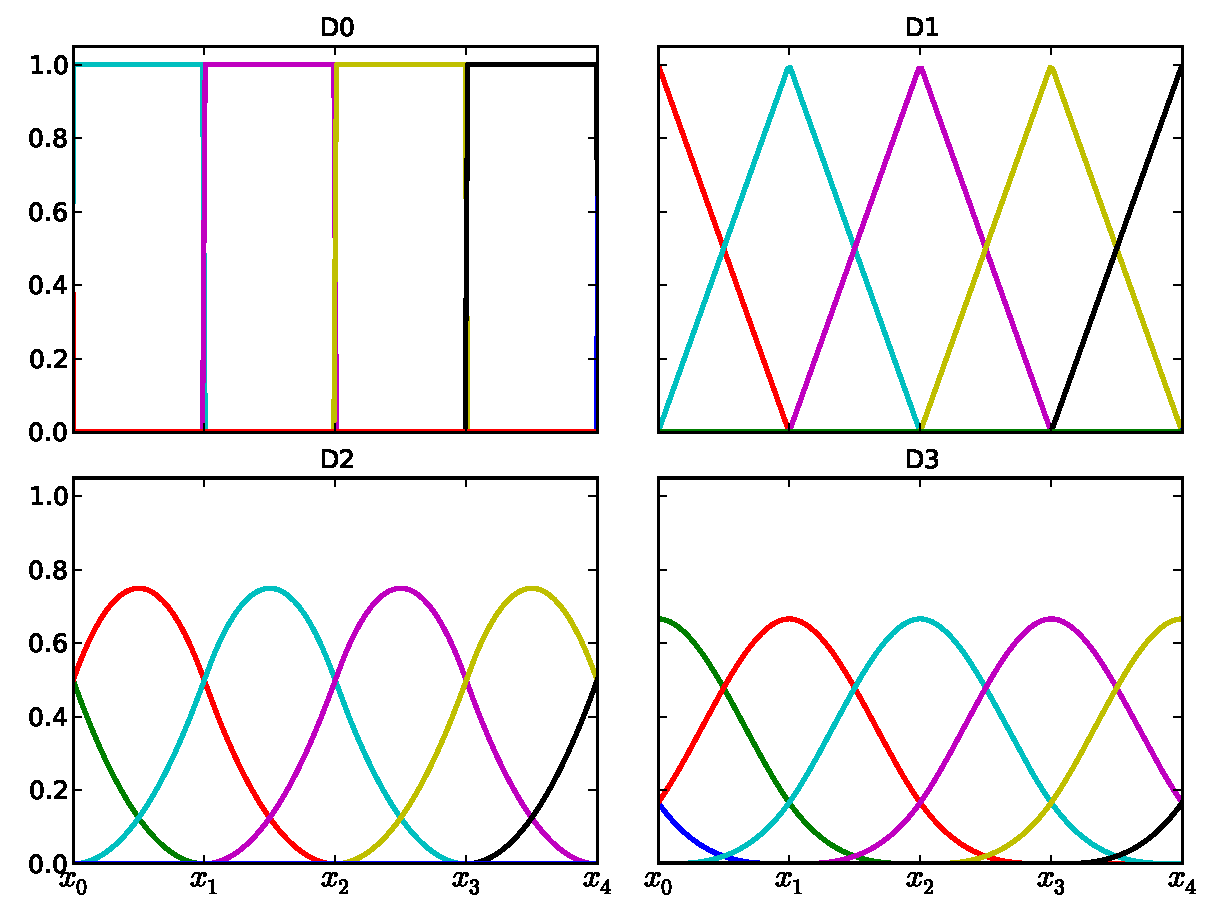
\includegraphics[scale=0.50]{BSplines_GeneralExpression_Deriv0.pdf}
    \caption{\small Bsplines of degrees 0, 1, 2 and 3}
    \label{Fig:Grid}
\end{figure}

A b-spline $b_{d,0}$ of degree $d$ living from $x_0$ is:$ b_{d,0} = \frac{x-x_0}{x_{0+d}-x_0}b_{d-1,0} + \frac{x_{0+d+1}-x}{x_{0+d+1}-x_{0+1}}b_{d-1,1} $\\
Hence:

$$
b_{0,0} =
\left\{
\begin{array}{lll}
1 & \text{ ,  if  } & x \in [x_0,x_1[\\
0 & \text{ ,  else}
\end{array}
\right.
$$

$$
b_{1,0} =
\left\{
\begin{array}{lll}
\frac{x-x_0}{x_1-x_0} & \text{ ,  if  } & x \in [x_0,x_1[\\
\frac{x_2-x}{x_2-x_1} & \text{ ,  if  } & x \in [x_1,x_2[
\end{array}
\right.
$$

$$
b_{2,0} =
\left\{
\begin{array}{lll}
\frac{(x-x_0)^2}{(x_2-x_0)(x_1-x_0)} & \text{ ,  if  } & x \in [x_0,x_1[\\
\frac{(x-x_0)(x_2-x)}{(x_2-x_0)(x_2-x_1)} + \frac{(x-x_1)(x_3-x)}{(x_2-x_1)(x_3-x_1)} & \text{ ,  if  } & x \in [x_1,x_2[\\
\frac{(x_3-x)^2}{(x_3-x_2)(x_3-x_1)} & \text{ ,  if  } & x \in [x_2,x_3[
\end{array}
\right.
$$

$$
b_{3,0} =
\left\{
\begin{array}{lll}
\frac{(x-x_0)^3}{(x_3-x_0)(x_2-x_0)(x_1-x_0)} & \text{ ,  if  } & x \in [x_0,x_1[\\
\frac{x-x_0}{x_3-x_0}\left(\frac{(x-x_0)(x_2-x)}{(x_2-x_0)(x_2-x_1)} + \frac{(x-x_1)(x_3-x)}{(x_2-x_1)(x_3-x_1)}\right) + \frac{x_4-x}{x_4-x_1}\left(\frac{(x-x_1)^2}{(x_3-x_1)(x_2-x_1)}\right) & \text{ ,  if  } & x \in [x_1,x_2[\\
\frac{x-x_0}{x_3-x_0}\left(\frac{(x_3-x)^2}{(x_3-x_2)(x_3-x_1)}\right) + \frac{x_4-x}{x_4-x_1}\left(\frac{(x-x_1)(x_3-x)}{(x_3-x_1)(x_3-x_2)} + \frac{(x-x_2)(x_4-x)}{(x_3-x_2)(x_4-x_2)}\right)& \text{ ,  if  } & x \in [x_2,x_3[\\
\frac{(x_4-x)^3}{(x_4-x_3)(x_4-x_2)(x_4-x_1)} & \text{ ,  if  } & x \in [x_3,x_4[
\end{array}
\right.
$$

Or (see \ref{Ap:DistribueDeg3} for details):

$$
b_{2,0} =
\left\{
\begin{array}{lll}
\frac{x^2-2xx_0+x_0^2}{(x_2-x_0)(x_1-x_0)} & \text{ ,  if  } & x \in [x_0,x_1[\\
\frac{-x^2(x_3+x_2-x_1-x_0) + 2x(x_3x_2-x_1x_0) - (x_3x_2x_0 - x_2x_1x_0 + x_3x_2x_1 - x_3x_1x_0)}{ (x_2-x_1)(x_2-x_0)(x_3-x_1)} & \text{ ,  if  } & x \in [x_1,x_2[\\
\frac{x^2-2xx_3+x_3^2}{(x_3-x_2)(x_3-x_1)} & \text{ ,  if  } & x \in [x_2,x_3[
\end{array}
\right.
$$


$$
b_{3,0} =
\left\{
\begin{array}{lll}
\frac{x^3 - 3x^2x_0 + 3xx_0^2 - x_0^3}{(x_3-x_0)(x_2-x_0)(x_1-x_0)} & \text{ ,  if  } & x \in [x_0,x_1[\\
\frac{x^3A + x^2B + xC + D}{(x_4-x_1)(x_3-x_1)(x_3-x_0)(x_2-x_1)(x_2-x_0)} & \text{ ,  if  } & x \in [x_1,x_2[\\
\frac{x^3A^/ + x^2B^/ + xC^/ + D^/}{(x_4-x_2)(x_4-x_1)(x_3-x_2)(x_3-x_1)(x_3-x_0)} & \text{ ,  if  } & x \in [x_2,x_3[\\
\frac{-x^3 + 3x^2x_4 - 3xx_4^2 + x_4^3}{(x_4-x_3)(x_4-x_2)(x_4-x_1)} & \text{ ,  if  } & x \in [x_3,x_4[
\end{array}
\right.
$$



\newpage
\section{Derivatives}

By noting $\partial_n b_{d,0}$ the $n$-th derivative of b-spline $b_{d,0}$, where $n\leq d$:

$$
\partial_1 b_{1,0} =
\left\{
\begin{array}{lll}
\frac{1}{x_1-x_0} & \text{ ,  if  } & x \in [x_0,x_1[\\
\frac{-1}{x_2-x_1} & \text{ ,  if  } & x \in [x_1,x_2[
\end{array}
\right.
$$

$$
\partial_1 b_{2,0} =
\left\{
\begin{array}{lll}
\frac{2(x-x_0)}{(x_2-x_0)(x_1-x_0)} & \text{ ,  if  } & x \in [x_0,x_1[\\
\frac{-2x(x_3+x_2-x_1-x_0) + 2(x_3x_2-x_1x_0)}{ (x_2-x_1)(x_2-x_0)(x_3-x_1)} & \text{ ,  if  } & x \in [x_1,x_2[\\
\frac{-2(x_3-x)}{(x_3-x_2)(x_3-x_1)} & \text{ ,  if  } & x \in [x_2,x_3[
\end{array}
\right.
$$

$$
\partial_2 b_{2,0} =
\left\{
\begin{array}{lll}
\frac{2}{(x_2-x_0)(x_1-x_0)} & \text{ ,  if  } & x \in [x_0,x_1[\\
\frac{-2(x_3+x_2-x_1-x_0)}{ (x_2-x_1)(x_2-x_0)(x_3-x_1)} & \text{ ,  if  } & x \in [x_1,x_2[\\
\frac{2}{(x_3-x_2)(x_3-x_1)} & \text{ ,  if  } & x \in [x_2,x_3[
\end{array}
\right.
$$


$$
\partial_1 b_{3,0} =
\left\{
\begin{array}{lll}
\frac{3(x-x_0)^2}{(x_3-x_0)(x_2-x_0)(x_1-x_0)} & \text{ ,  if  } & x \in [x_0,x_1[\\
\frac{3x^2A + 2xB + C}{(x_4-x_1)(x_3-x_1)(x_3-x_0)(x_2-x_1)(x_2-x_0)} & \text{ ,  if  } & x \in [x_1,x_2[\\
\frac{3x^2A^/ + 2xB^/ + C^/}{(x_4-x_2)(x_4-x_1)(x_3-x_2)(x_3-x_1)(x_3-x_0)} & \text{ ,  if  } & x \in [x_2,x_3[\\
\frac{-3(x_4-x)^2}{(x_4-x_3)(x_4-x_2)(x_4-x_1)} & \text{ ,  if  } & x \in [x_3,x_4[
\end{array}
\right.
$$

$$
\partial_2 b_{3,0} =
\left\{
\begin{array}{lll}
\frac{6(x-x_0)}{(x_3-x_0)(x_2-x_0)(x_1-x_0)} & \text{ ,  if  } & x \in [x_0,x_1[\\
\frac{6xA + 2B}{(x_4-x_1)(x_3-x_1)(x_3-x_0)(x_2-x_1)(x_2-x_0)} & \text{ ,  if  } & x \in [x_1,x_2[\\
\frac{6xA^/ + 2B^/}{(x_4-x_2)(x_4-x_1)(x_3-x_2)(x_3-x_1)(x_3-x_0)} & \text{ ,  if  } & x \in [x_2,x_3[\\
\frac{6(x_4-x)}{(x_4-x_3)(x_4-x_2)(x_4-x_1)} & \text{ ,  if  } & x \in [x_3,x_4[
\end{array}
\right.
$$

$$
\partial_3 b_{3,0} =
\left\{
\begin{array}{lll}
\frac{6}{(x_3-x_0)(x_2-x_0)(x_1-x_0)} & \text{ ,  if  } & x \in [x_0,x_1[\\
\frac{6A}{(x_4-x_1)(x_3-x_1)(x_3-x_0)(x_2-x_1)(x_2-x_0)} & \text{ ,  if  } & x \in [x_1,x_2[\\
\frac{6A^/}{(x_4-x_2)(x_4-x_1)(x_3-x_2)(x_3-x_1)(x_3-x_0)} & \text{ ,  if  } & x \in [x_2,x_3[\\
\frac{-6}{(x_4-x_3)(x_4-x_2)(x_4-x_1)} & \text{ ,  if  } & x \in [x_3,x_4[
\end{array}
\right.
$$







\newpage
\begin{landscape}

\begin{figure}[hbtp]
    \centering
    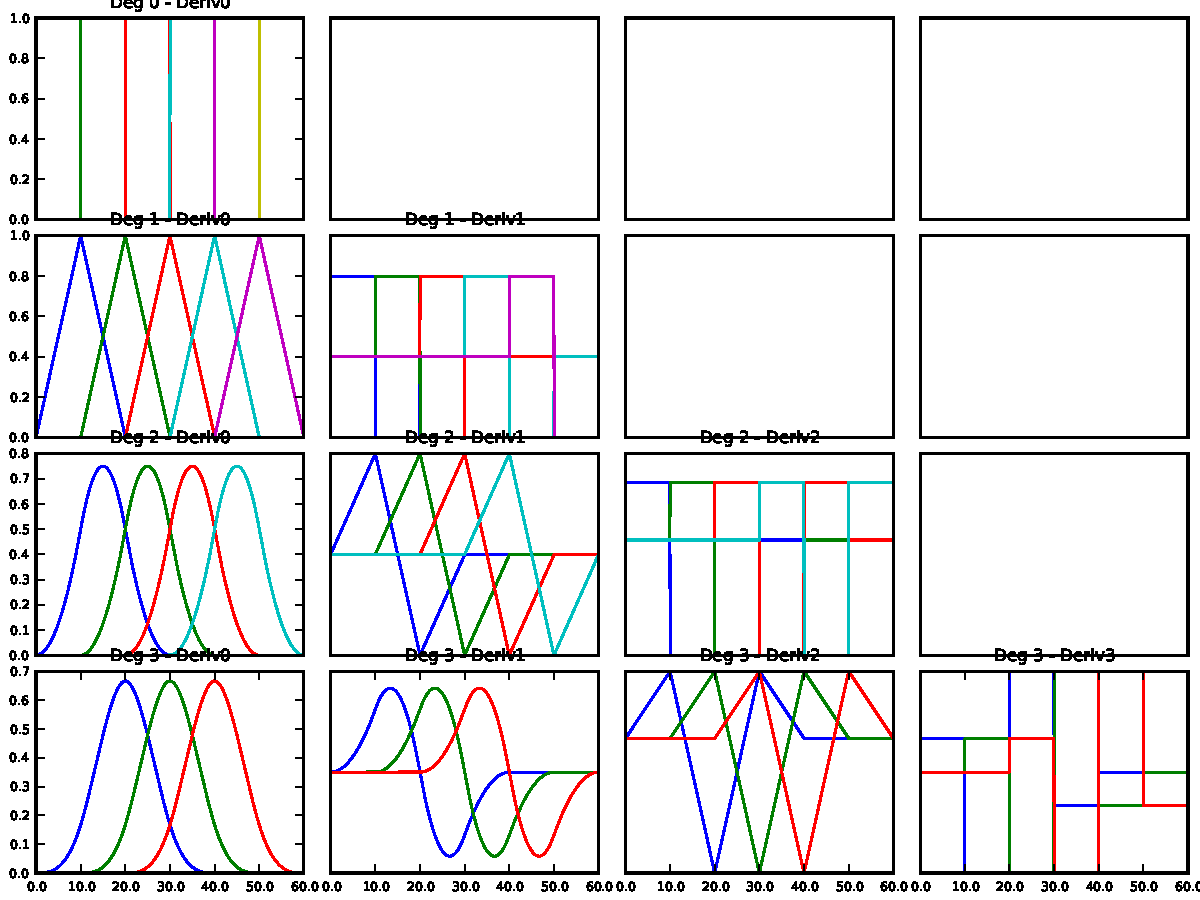
\includegraphics[scale=0.75]{tests01_bsplines_test02_BSpline_LFunc.pdf}
    \caption{\small Bsplines of degrees 0, 1, 2 and 3 and their derivatives D0, D1, D2 and D3}
    \label{Fig:Deriv}
\end{figure}


\newpage
\appendix

\section{Distributing the degree 3 polynoms}
\label{Ap:DistribueDeg3}

$$
\begin{array}{ll}
& \frac{x-x_0}{x_3-x_0}\left(\frac{(x-x_0)(x_2-x)}{(x_2-x_0)(x_2-x_1)} + \frac{(x-x_1)(x_3-x)}{(x_2-x_1)(x_3-x_1)}\right) + \frac{x_4-x}{x_4-x_1}\left(\frac{(x-x_1)^2}{(x_3-x_1)(x_2-x_1)}\right)\\
= & \frac{ (x-x_0)^2(x_2-x)(x_3-x_1)(x_4-x_1) + (x-x_0)(x-x_1)(x_3-x)(x_2-x_0)(x_4-x_1) + (x_4-x)(x-x_1)^2(x_3-x_0)(x_2-x_0) }{(x_4-x_1)(x_3-x_1)(x_3-x_0)(x_2-x_1)(x_2-x_0)}\\
= & \frac{ (x^2-2xx_0+x_0^2)(x_2-x)(x_3-x_1)(x_4-x_1) + (x^2-x(x_0+x_1)+x_0x_1)(x_3-x)(x_2-x_0)(x_4-x_1) + (x^2-2xx_1+x_1^2)(x_4-x)(x_3-x_0)(x_2-x_0) }{(x_4-x_1)(x_3-x_1)(x_3-x_0)(x_2-x_1)(x_2-x_0)}\\

= & \frac{ (x^2x_2-2xx_2x_0+x_2x_0^2 - x^3+2x^2x_0-xx_0^2)(x_3-x_1)(x_4-x_1) + (x^2x_3-xx_3(x_0+x_1)+x_0x_1x_3 - x^3+x^2(x_0+x_1)-xx_0x_1)(x_2-x_0)(x_4-x_1)
+ (x^2x_4-2xx_4x_1+x_4x_1^2 - x^3+2x^2x_1-xx_1^2)(x_3-x_0)(x_2-x_0) }{(x_4-x_1)(x_3-x_1)(x_3-x_0)(x_2-x_1)(x_2-x_0)}\\

= & \frac{1}{(x_4-x_1)(x_3-x_1)(x_3-x_0)(x_2-x_1)(x_2-x_0)} \left[ \begin{array}{ll}
-x^3((x_3-x_1)(x_4-x_1) + (x_2-x_0)(x_4-x_1) + (x_3-x_0)(x_2-x_0))\\
+ x^2( (x_2+2x_0)(x_3-x_1)(x_4-x_1) + (x_3+x_0+x_1)(x_2-x_0)(x_4-x_1) + (x_4+2x_1)(x_3-x_0)(x_2-x_0) )\\
+ x( -x_0(2x_2+x_0)(x_3-x_1)(x_4-x_1) - (x_3(x_0+x_1)+x_0x_1)(x_2-x_0)(x_4-x_1) - x_1(2x_4+x_1)(x_3-x_0)(x_2-x_0) )\\
+ x_2x_0^2(x_3-x_1)(x_4-x_1) + x_0x_1x_3(x_2-x_0)(x_4-x_1) + x_4x_1^2(x_3-x_0)(x_2-x_0)
\end{array}\right]\\

= & \frac{ Ax^3 + Bx^2 + Cx + D }{(x_4-x_1)(x_3-x_1)(x_3-x_0)(x_2-x_1)(x_2-x_0)}

\end{array}
$$

where $\left\{\begin{array}{ll}
A & = -((x_3-x_1)(x_4-x_1) + (x_2-x_0)(x_4-x_1) + (x_3-x_0)(x_2-x_0))\\
B & = (x_2+2x_0)(x_3-x_1)(x_4-x_1) + (x_3+x_0+x_1)(x_2-x_0)(x_4-x_1) + (x_4+2x_1)(x_3-x_0)(x_2-x_0)\\
C & = -(x_0(2x_2+x_0)(x_3-x_1)(x_4-x_1) + (x_3(x_0+x_1)+x_0x_1)(x_2-x_0)(x_4-x_1) + x_1(2x_4+x_1)(x_3-x_0)(x_2-x_0))\\
D & = x_2x_0^2(x_3-x_1)(x_4-x_1) + x_0x_1x_3(x_2-x_0)(x_4-x_1) + x_4x_1^2(x_3-x_0)(x_2-x_0)
\end{array}\right.$\\




Similarly
$$
\frac{x-x_0}{x_3-x_0}\left(\frac{(x_3-x)^2}{(x_3-x_2)(x_3-x_1)}\right) + \frac{x_4-x}{x_4-x_1}\left(\frac{(x-x_1)(x_3-x)}{(x_3-x_1)(x_3-x_2)} + \frac{(x-x_2)(x_4-x)}{(x_3-x_2)(x_4-x_2)}\right)
= \frac{x^3A^/ + x^2B^/ + xC^/ + D^/}{(x_4-x_2)(x_4-x_1)(x_3-x_2)(x_3-x_1)(x_3-x_0)}
$$

where we simply substitute $(x_0,x_1,x_2,x_3,x_4)$ in $A,B,C,D$ by $(x_4,x_3,x_2,x_1,x_0)$ and notice that the denominator is the opposite of the substituted version:
$$
\left\{\begin{array}{ll}
A^/ & = (x_1-x_3)(x_0-x_3) + (x_2-x_4)(x_0-x_3) + (x_1-x_4)(x_2-x_4)\\
B^/ & = -((x_2+2x_4)(x_1-x_3)(x_0-x_3) + (x_1+x_4+x_3)(x_2-x_4)(x_0-x_3) + (x_0+2x_3)(x_1-x_4)(x_2-x_4))\\
C^/ & = x_4(2x_2+x_4)(x_1-x_3)(x_0-x_3) + (x_1(x_4+x_3)+x_4x_3)(x_2-x_4)(x_0-x_3) + x_3(2x_0+x_3)(x_1-x_4)(x_2-x_4)\\
D^/ & = -(x_2x_4^2(x_1-x_3)(x_0-x_3) + x_4x_3x_1(x_2-x_4)(x_0-x_3) + x_0x_3^2(x_1-x_4)(x_2-x_4))
\end{array}\right.
$$


\end{landscape}









%%% End document
\end{document}
